\documentclass[handout,nooutcomes,noauthor]{ximera}

\graphicspath{  
{./}
{./whoAreYou/}
{./drawingWithTheTurtle/}
{./bisectionMethod/}
{./circles/}
{./anglesAndRightTriangles/}
{./lawOfSines/}
{./lawOfCosines/}
{./plotter/}
{./staircases/}
{./pitch/}
{./qualityControl/}
{./symmetry/}
{./nGonBlock/}
}


%% page layout
\usepackage[cm,headings]{fullpage}
\raggedright
\setlength\headheight{13.6pt}


%% fonts
\usepackage{euler}

\usepackage{FiraMono}
\renewcommand\familydefault{\ttdefault} 
\usepackage[defaultmathsizes]{mathastext}
\usepackage[htt]{hyphenat}

\usepackage[T1]{fontenc}
\usepackage[scaled=1]{FiraSans}

%\usepackage{wedn}
\usepackage{pbsi} %% Answer font


\usepackage{cancel} %% strike through in pitch/pitch.tex


%% \usepackage{ulem} %% 
%% \renewcommand{\ULthickness}{2pt}% changes underline thickness

\tikzset{>=stealth}

\usepackage{adjustbox}

\setcounter{titlenumber}{-1}

%% journal style
\makeatletter
\newcommand\journalstyle{%
  \def\activitystyle{activity-chapter}
  \def\maketitle{%
    \addtocounter{titlenumber}{1}%
                {\flushleft\small\sffamily\bfseries\@pretitle\par\vspace{-1.5em}}%
                {\flushleft\LARGE\sffamily\bfseries\thetitlenumber\hspace{1em}\@title \par }%
                {\vskip .6em\noindent\textit\theabstract\setcounter{question}{0}\setcounter{sectiontitlenumber}{0}}%
                    \par\vspace{2em}
                    \phantomsection\addcontentsline{toc}{section}{\thetitlenumber\hspace{1em}\textbf{\@title}}%
                     }}
\makeatother



%% thm like environments
\let\question\relax
\let\endquestion\relax

\newtheoremstyle{QuestionStyle}{\topsep}{\topsep}%%% space between body and thm
		{}                      %%% Thm body font
		{}                              %%% Indent amount (empty = no indent)
		{\bfseries}            %%% Thm head font
		{)}                              %%% Punctuation after thm head
		{ }                           %%% Space after thm head
		{\thmnumber{#2}\thmnote{ \bfseries(#3)}}%%% Thm head spec
\theoremstyle{QuestionStyle}
\newtheorem{question}{}



\let\freeResponse\relax
\let\endfreeResponse\relax

%% \newtheoremstyle{ResponseStyle}{\topsep}{\topsep}%%% space between body and thm
%% 		{\wedn\bfseries}                      %%% Thm body font
%% 		{}                              %%% Indent amount (empty = no indent)
%% 		{\wedn\bfseries}            %%% Thm head font
%% 		{}                              %%% Punctuation after thm head
%% 		{3ex}                           %%% Space after thm head
%% 		{\underline{\underline{\thmname{#1}}}}%%% Thm head spec
%% \theoremstyle{ResponseStyle}

\usepackage[tikz]{mdframed}
\mdfdefinestyle{ResponseStyle}{leftmargin=1cm,linecolor=black,roundcorner=5pt,
, font=\bsifamily,}%font=\wedn\bfseries\upshape,}


\ifhandout
\NewEnviron{freeResponse}{}
\else
%\newtheorem{freeResponse}{Response:}
\newenvironment{freeResponse}{\begin{mdframed}[style=ResponseStyle]}{\end{mdframed}}
\fi



%% attempting to automate outcomes.

%% \newwrite\outcomefile
%%   \immediate\openout\outcomefile=\jobname.oc
%% \renewcommand{\outcome}[1]{\edef\theoutcomes{\theoutcomes #1~}%
%% \immediate\write\outcomefile{\unexpanded{\outcome}{#1}}}

%% \newcommand{\outcomelist}{\begin{itemize}\theoutcomes\end{itemize}}

%% \NewEnviron{listOutcomes}{\small\sffamily
%% After answering the following questions, students should be able to:
%% \begin{itemize}
%% \BODY
%% \end{itemize}
%% }
\usepackage[tikz]{mdframed}
\mdfdefinestyle{OutcomeStyle}{leftmargin=2cm,rightmargin=2cm,linecolor=black,roundcorner=5pt,
, font=\small\sffamily,}%font=\wedn\bfseries\upshape,}
\newenvironment{listOutcomes}{\begin{mdframed}[style=OutcomeStyle]After answering the following questions, students should be able to:\begin{itemize}}{\end{itemize}\end{mdframed}}



%% my commands

\newcommand{\snap}{{\bfseries\itshape\textsf{Snap!}}}
\newcommand{\flavor}{\link[\snap]{https://snap.berkeley.edu/}}
\newcommand{\mooculus}{\textsf{\textbf{MOOC}\textnormal{\textsf{ULUS}}}}


\usepackage{tkz-euclide}
\tikzstyle geometryDiagrams=[rounded corners=.5pt,ultra thick,color=black]
\colorlet{penColor}{black} % Color of a curve in a plot



\ifhandout\newcommand{\mynewpage}{\newpage}\else\newcommand{\mynewpage}{}\fi


\title{All you need are reflections}
\author{Bart Snapp}

\begin{document}
\begin{abstract}
  All rotations can be viewed as a composition of reflections.
\end{abstract}
\maketitle

\noindent\textbf{Group members (please print):}\ \hrulefill \\

\hrulefill

In this activity, we are going to explore how reflections are related
to rotations. When doing this activity, you don't need to worry about
the actual matrices involved, instead express your answers in terms of
reflections across lines, for example $\mat{F}_{x=4}$ is the
reflection across the vertical line $x=4$.

\begin{problem}
You may have noticed that $180^\circ$ rotations and horizontal (or
vertical) reflections seem kind of similar. Explain how they are
similar, then explain how they are different.
\end{problem}


\begin{problem}
Explain how to express a $180^\circ$ rotation as the composition of two
reflections. Work out some examples to give evidence that you are
correct.
\end{problem}
Consider the following ``F'' shape:
\[
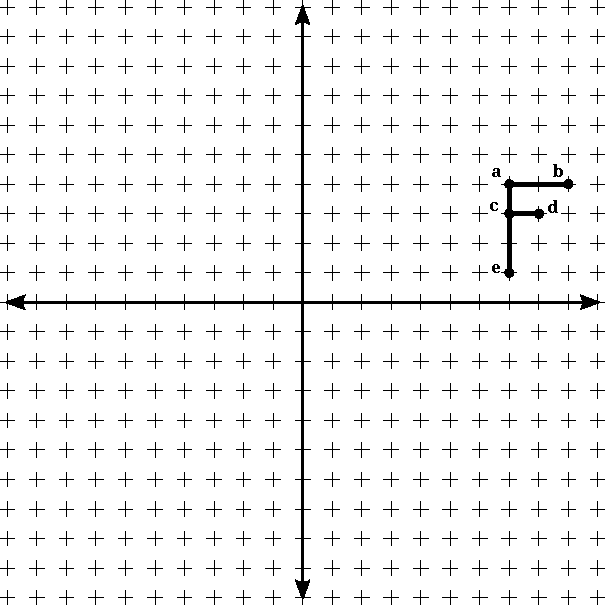
\includegraphics{planeR.pdf}
\]
\begin{problem}
Reflect our shape across the line $y=x$. Label the reflection of the
points with a prime---the reflection of $\mathbf{a}$ across $y=x$ is
$\mathbf{a}'$.
\end{problem}

\begin{problem}
Reflect our new shape across $x=0$. Label the reflection of the points
with another prime---the reflection of $\mathbf{a}'$ across $x=0$ is
$\mathbf{a}''$.
\end{problem}

\begin{problem}
Through how many degrees was our original shape rotated about the
origin?
\end{problem}


\begin{problem}
Letting $\mathbf{o}$ be the origin and ``$-$'' be a place holder, use
a protractor to fill in the described angles:
\[
{\renewcommand{\arraystretch}{2}
\begin{array}{|c|c|c|c|}\hline
- & -, \ \mathbf{o}, \text{ and }-' & -',\ \mathbf{o},\text{ and }-'' & \ -, \mathbf{o},\text{ and }-'' \\ \hline\hline
\mathbf{a} & & & \\ \hline 
\mathbf{b} & & & \\ \hline 
\mathbf{c} & & & \\ \hline  
\mathbf{d} & & & \\ \hline  
\mathbf{e} & & & \\ \hline        
\end{array}}
\]
What do you notice?
\end{problem}



\begin{problem}
Letting $\mathbf{o}$ be the origin and ``$-$'' be a place holder, use
a protractor to fill in the described angles:
\[
{\renewcommand{\arraystretch}{2}
\begin{array}{|c|c|c|c|}\hline
- & -,\ \mathbf{o}, \text{ and }y=x &  -', \ \mathbf{o}, \text{ and }x=0 & \text{the sum} \\ \hline\hline
\mathbf{a} & & & \\ \hline 
\mathbf{b} & & & \\ \hline 
\mathbf{c} & & & \\ \hline  
\mathbf{d} & & & \\ \hline  
\mathbf{e} & & & \\ \hline        
\end{array}}
\]
What do you notice?
\end{problem}


\begin{problem}
Suppose I want to rotate an object $\theta^\circ$ around the origin
using two reflections. Can you conjecture how the lines should be
placed on the plane? Draw pictures to help with your explanation.
\end{problem}

\end{document}
